\section{Robustness under Distribution Shift}
\label{sec:distribution_shift}

The previous experiments evaluate forecasting performance over the complete
test distribution. However, average performance may hide substantial
degradation under traffic conditions that are less frequently represented
during training. To investigate this aspect, the Graph-Temporal model is
evaluated under a predefined high-congestion stress condition. The stress
condition is defined exclusively from the training data, preventing
information from the validation or test sets from influencing the definition
of the shifted subset.

\subsection{High-Congestion Definition}
\label{subsec:congestion_definition}

High-congestion conditions are identified using sensor-specific speed
thresholds. For each sensor $n$, a congestion threshold $\tau_n$ is defined
as the 10th percentile of its valid speed observations in the training set,

\begin{equation}
    \tau_n =
    Q_{0.10}
    \left(
        \left\{y_{t,n}^{\mathrm{train}} :
        m_{t,n}^{\mathrm{train}} = 1\right\}
    \right),
    \label{eq:sensor_congestion_threshold}
\end{equation}

where $m_{t,n}^{\mathrm{train}}$ denotes the availability mask. A sensor is
therefore considered congested at time $t$ when its valid observed speed is
lower than or equal to its sensor-specific threshold. Using a separate
threshold for each sensor accounts for the different typical speed ranges
observed across locations in the road network.

The network-level congestion ratio at timestamp $t$ is then defined as the
fraction of valid sensors that are classified as congested,

\begin{equation}
    C_t =
    \frac{
        \sum_{n=1}^{N}
        m_{t,n}\,
        \mathbb{I}\!\left(y_{t,n} \leq \tau_n\right)
    }{
        \sum_{n=1}^{N} m_{t,n}
    },
    \label{eq:congestion_ratio}
\end{equation}

where $\mathbb{I}(\cdot)$ is the indicator function. This definition measures
the spatial extent of congestion at each timestamp rather than relying on the
speed of a single sensor.

Finally, the threshold used to identify a high-congestion event is defined
as the 95th percentile of the congestion ratios observed in the training
set,

\begin{equation}
    \tau_{\mathrm{peak}}
    =
    Q_{0.95}
    \left(
        \left\{C_t^{\mathrm{train}}\right\}
    \right).
    \label{eq:peak_threshold}
\end{equation}

For the METR-LA training partition, this procedure yields
$\tau_{\mathrm{peak}} = 0.3495$. Consequently, a timestamp is classified as
a high-congestion condition when at least approximately 35\% of the valid
sensors simultaneously exhibit speeds below their respective training-based
10th-percentile thresholds.

\begin{figure}[t]
    \centering
    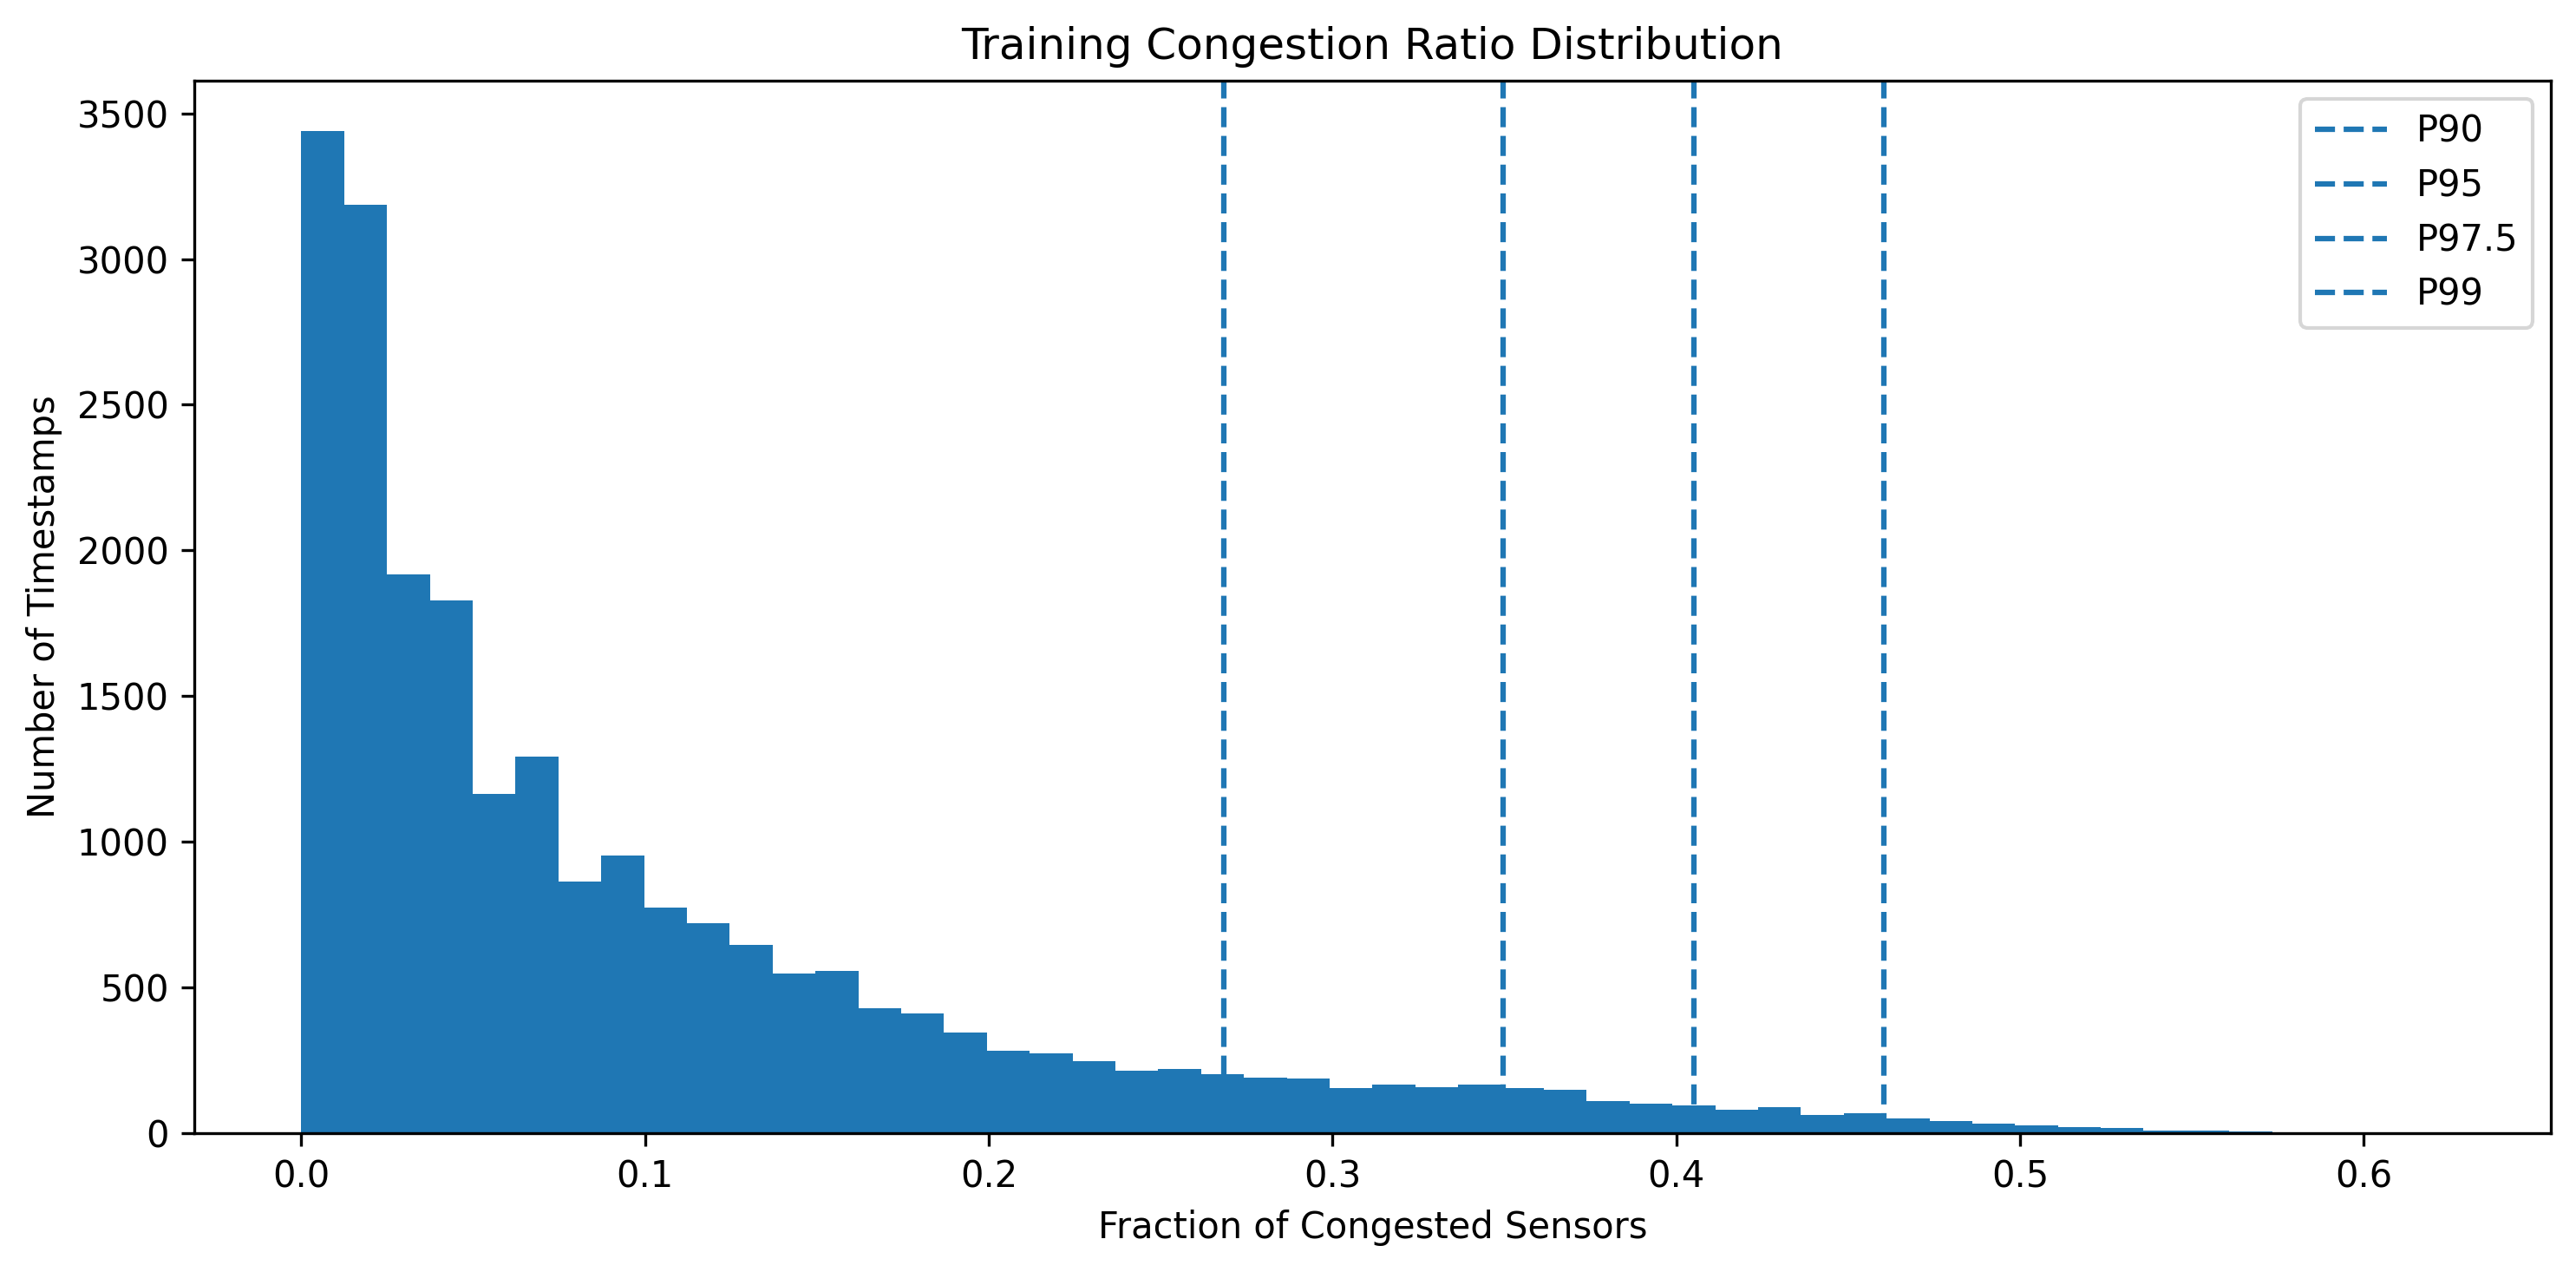
\includegraphics[width=0.75\linewidth]
    {img/distribution_shift/congestion_ratio_distribution}
    \caption{Distribution of the network-level congestion ratio $C_t$ in the
    training set.}
    \label{fig:congestion_ratio_distribution}
\end{figure}

Figure~\ref{fig:congestion_ratio_distribution} shows the training
distribution used to define the stress condition. By selecting its 95th
percentile, the stress test focuses on relatively uncommon periods in which
congestion simultaneously affects a substantial fraction of the network.
Importantly, both the sensor-specific thresholds $\tau_n$ and the
network-level threshold $\tau_{\mathrm{peak}}$ are estimated exclusively
from the training partition and subsequently kept fixed when classifying
validation and test observations.


\subsection{Stress-Test Protocol}
\label{subsec:stress_protocol}

The high-congestion definition introduced in
Section~\ref{subsec:congestion_definition} is applied to the forecasting
targets of each test window. Since the model is evaluated at three different
forecasting horizons, congestion is assessed independently at the target
timestamp corresponding to each horizon.

More specifically, for a test sample whose input sequence ends at time $t$,
the congestion condition for forecasting horizon $h$ is determined from the
network-level congestion ratio at the corresponding future timestamp
$t+h$. The sample is classified as high congestion for horizon $h$ when

\begin{equation}
    C_{t+h} \geq \tau_{\mathrm{peak}},
    \label{eq:high_congestion_sample}
\end{equation}

where $\tau_{\mathrm{peak}}=0.3495$ is the threshold estimated exclusively
from the training partition. Otherwise, the sample is assigned to the normal
subset for that horizon.

This horizon-specific classification is necessary because traffic conditions
may change within the 60-minute forecasting window. Consequently, the same
input window can be classified as normal at one forecasting horizon and as
high congestion at another. The stress-test subsets for 15, 30, and
60 minutes should therefore be interpreted independently rather than as a
single fixed set of test windows.

Applying this procedure to the 6224 test windows yields 484 high-congestion
samples and 5740 normal samples at each evaluated horizon. Although the
subset sizes are identical, their composition differs across horizons. For
example, the high-congestion masks have a Jaccard similarity of 0.741 between
15 and 30 minutes, 0.579 between 30 and 60 minutes, and 0.449 between
15 and 60 minutes. This decreasing overlap is expected because the target
timestamps become progressively farther apart.

The stress test evaluates the same trained Graph-Temporal model used in the
previous experiments, without retraining or adapting it to high-congestion
conditions. Forecasting metrics are computed separately over the normal and
high-congestion subsets using the target availability mask. This allows the
degradation associated with the shifted traffic condition to be measured
while keeping the model, preprocessing pipeline, and evaluation procedure
unchanged.

\subsection{Quantitative Results}
\label{subsec:shift_quantitative}

Table~\ref{tab:congestion_results} reports the performance of the
Graph-Temporal model separately under normal and high-congestion conditions.
A substantial degradation is observed under high congestion at all three
forecasting horizons, and the difference becomes progressively larger as the
prediction horizon increases.

\begin{table}[t]
    \centering
    \caption{Performance of the Graph-Temporal model under normal and
    high-congestion conditions on the test set.}
    \label{tab:congestion_results}
    \begin{tabular}{llrrrr}
        \toprule
        Condition & Horizon &
        MAE & RMSE & Coverage (\%) & Interval Width \\
        \midrule
        Normal
        & 15 min & 2.770 & 5.289 & 78.4 & 8.499 \\
        & 30 min & 3.257 & 6.453 & 78.3 & 9.911 \\
        & 60 min & 3.974 & 7.957 & 78.3 & 11.730 \\
        \midrule
        High congestion
        & 15 min & 4.463 & 7.669 & 78.7 & 14.035 \\
        & 30 min & 5.636 & 9.660 & 77.9 & 17.283 \\
        & 60 min & 7.414 & 12.296 & 75.8 & 21.169 \\
        \bottomrule
    \end{tabular}
\end{table}

It is worth noting that the performance observed under normal conditions is
close to the overall test performance reported in
Section~\ref{sec:in_distribution_results}. This is expected from the
definition of the stress condition. High congestion is intentionally defined
as a relatively rare event through the 95th percentile of the training
congestion-ratio distribution and accounts for only 484 out of 6,224 test
windows, approximately 7.8\%, at each forecasting horizon. Consequently,
the overall test metrics are dominated by the much larger normal subset and
can therefore conceal the substantially poorer performance observed during
high-congestion periods.

\begin{figure}[t]
    \centering

    % First row: point forecasting metrics
    \begin{minipage}[b]{0.48\linewidth}
        \centering
        
\includegraphics[width=\linewidth]
        {img/distribution_shift/mae_distribution_shift}
    \end{minipage}
    \hfill
    \begin{minipage}[b]{0.48\linewidth}
        \centering
        
\includegraphics[width=\linewidth]
        {img/distribution_shift/rmse_distribution_shift}
    \end{minipage}

    \vspace{0.4cm}

    % Second row: probabilistic metrics
    \begin{minipage}[b]{0.48\linewidth}
        \centering
        
\includegraphics[width=\linewidth]
        {img/distribution_shift/coverage_distribution_shift}
    \end{minipage}
    \hfill
    \begin{minipage}[b]{0.48\linewidth}
        \centering
        
\includegraphics[width=\linewidth]
        {img/distribution_shift/interval_width_distribution_shift}
    \end{minipage}

    \caption{Performance of the Graph-Temporal model under normal and
    high-congestion conditions. The top row compares MAE (left) and RMSE
    (right), while the bottom row reports empirical coverage (left) and
    prediction interval width (right) across the three forecasting horizons.}
    \label{fig:congestion_performance}
\end{figure}

The degradation in point forecasting accuracy is clearly visible in
Figure~\ref{fig:congestion_performance}. At 15 minutes, MAE increases from
2.770 under normal conditions to 4.463 under high congestion, corresponding
to an increase of approximately 61\%. The difference becomes larger at
longer horizons: MAE increases from 3.257 to 5.636 at 30 minutes and from
3.974 to 7.414 at 60 minutes, corresponding to increases of approximately
73\% and 87\%, respectively. RMSE exhibits the same behavior, increasing
from 5.289 to 7.669, from 6.453 to 9.660, and from 7.957 to 12.296.
These results show that forecasting becomes substantially more difficult
during network-wide congestion and that the performance degradation becomes
more pronounced as the forecasting horizon increases.

The prediction intervals respond to the increased forecasting difficulty by
becoming substantially wider under high congestion. Their average width
increases from 8.499 to 14.035 at 15 minutes, from 9.911 to 17.283 at
30 minutes, and from 11.730 to 21.169 at 60 minutes. The model therefore
captures part of the increased uncertainty associated with congested traffic
conditions rather than maintaining intervals of approximately constant width.

However, the increase in interval width is not sufficient to preserve
calibration at the longest forecasting horizon. At 15 minutes, empirical
coverage remains approximately stable, changing from 78.4\% under normal
conditions to 78.7\% under high congestion. At 30 minutes, it decreases
slightly from 78.3\% to 77.9\%. The largest degradation occurs at 60 minutes,
where coverage decreases from approximately 78.3\% to 75.8\%, despite the
prediction intervals being substantially wider. Relative to the nominal
80\% coverage level, this indicates increased undercoverage during
high-congestion periods at the longest forecasting horizon.

Overall, the stress test reveals two distinct effects of high-congestion
conditions. First, point forecasting errors increase substantially, showing
that these traffic regimes are more difficult to predict than normal
conditions. Second, although the model reacts to this increased difficulty
by producing wider prediction intervals, the uncertainty estimates do not
fully compensate for the degradation at longer horizons. In particular, the
combination of substantially wider intervals and lower coverage at 60 minutes
indicates residual overconfidence under distribution shift. This motivates
the calibration mitigation investigated in Section~\ref{sec:mitigation}.

\subsection{Qualitative Analysis}
\label{subsec:shift_qualitative}

The aggregate behavior observed in the stress test is further examined
through representative forecasting examples. Figure~\ref{fig:shift_examples}
compares predictions produced by the Graph-Temporal model under normal and
high-congestion conditions. The examples are intended to illustrate how the
changes in forecasting accuracy and predictive uncertainty identified in the
quantitative analysis appear at the level of individual forecasting windows.

\begin{figure}[t]
    \centering

    \begin{minipage}[b]{0.49\linewidth}
        \centering
        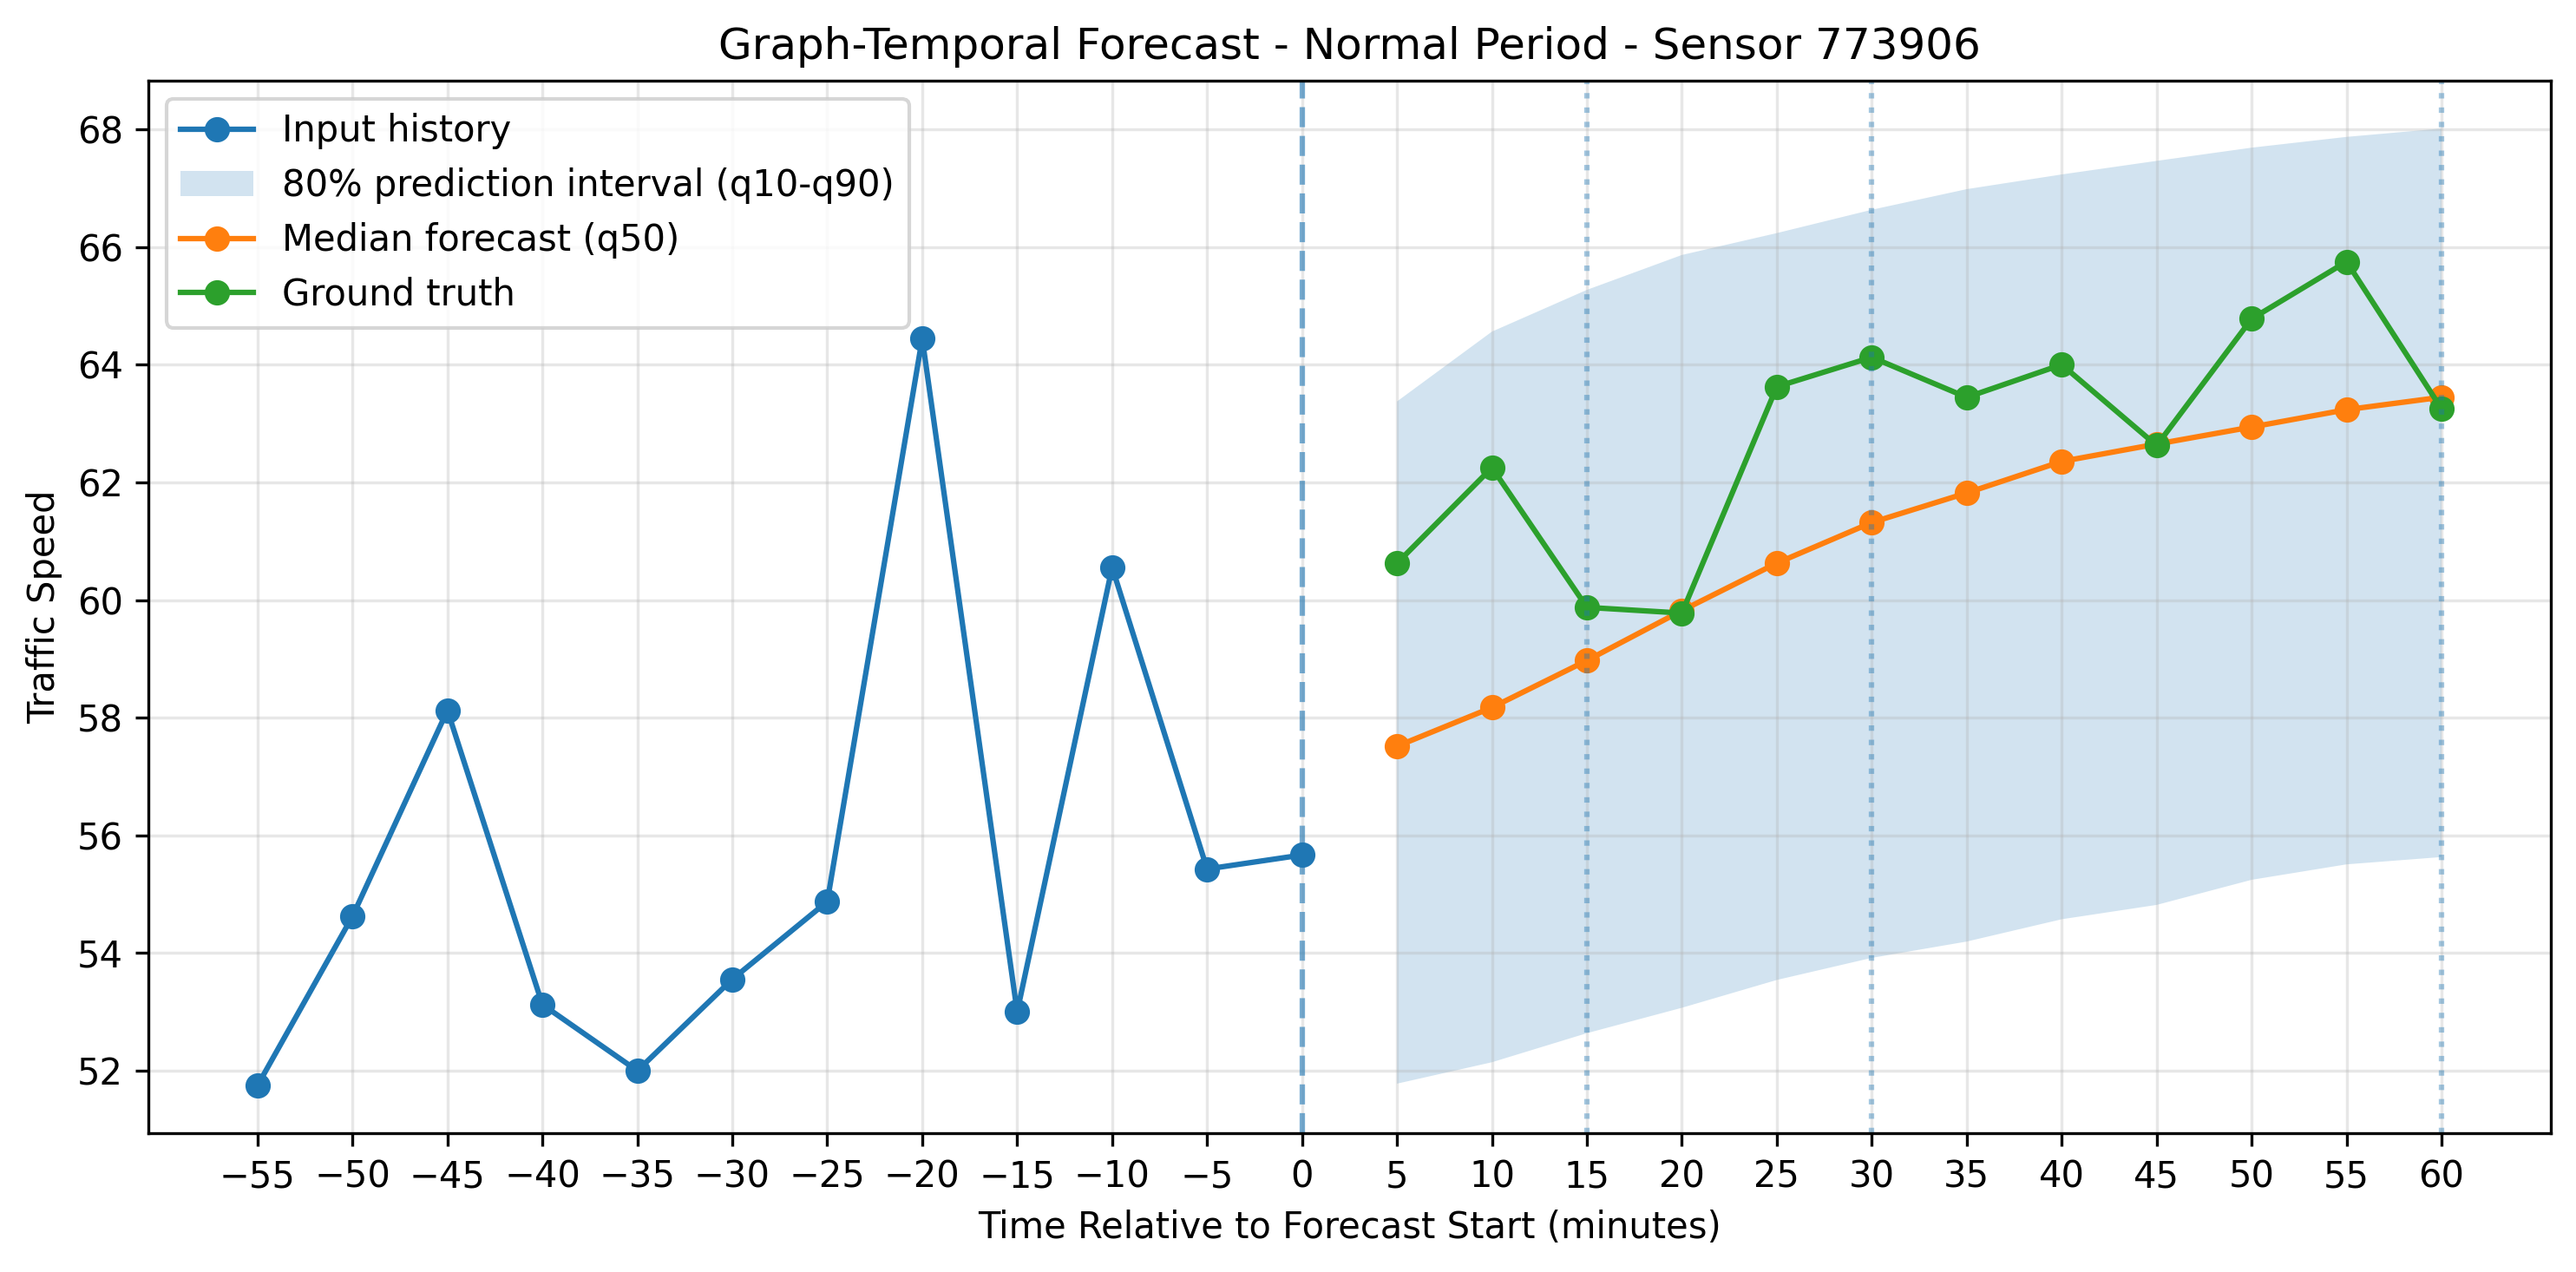
\includegraphics[width=\linewidth]
        {img/distribution_shift/normal_period}
    \end{minipage}
    \hfill
    \begin{minipage}[b]{0.49\linewidth}
        \centering
        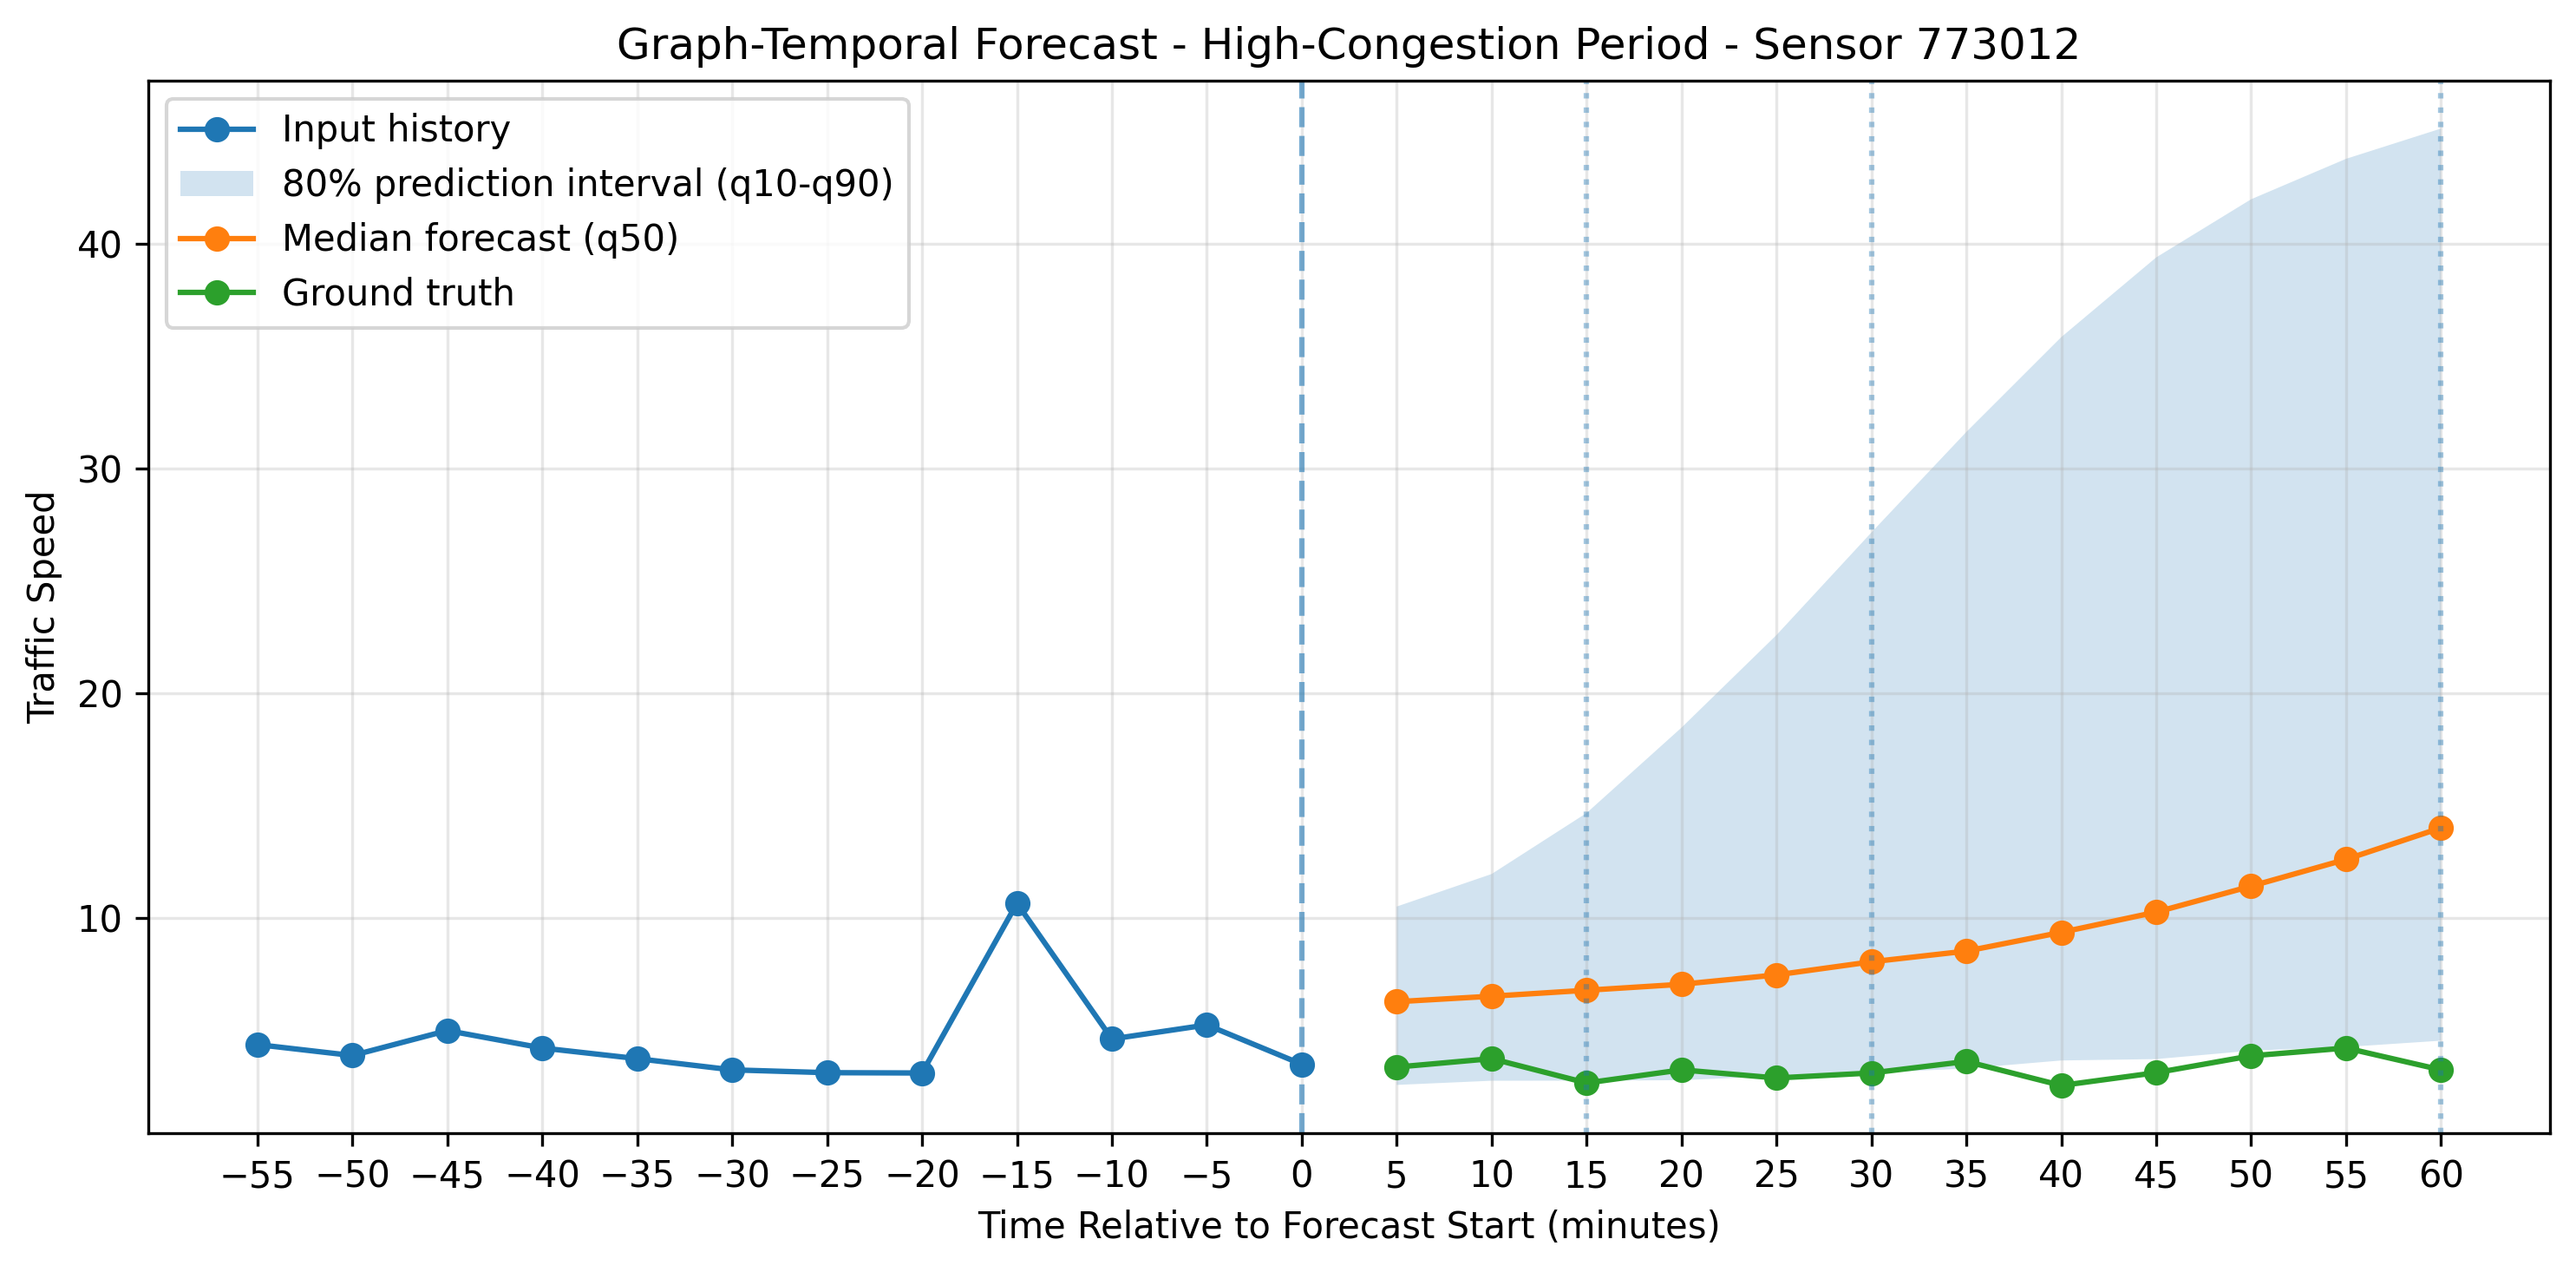
\includegraphics[width=\linewidth]
        {img/distribution_shift/high_congestion_period}
    \end{minipage}

    \caption{Representative probabilistic forecasts produced by the
    Graph-Temporal model under normal (left) and high-congestion (right)
    conditions.}
    \label{fig:shift_examples}
\end{figure}

Figure~\ref{fig:shift_examples} provides a qualitative view of how the
forecasting behavior changes between normal and high-congestion conditions.
In the normal example (left), traffic speeds remain relatively high and the
model successfully captures the increasing trend observed over the forecasting
window. Although the median forecast does not reproduce every short-term
fluctuation of the ground truth, it follows its overall evolution, while the
prediction interval remains moderately wide and contains the observed values
throughout most of the horizon.

A markedly different behavior emerges in the high-congestion example (right).
The very low observed speeds reflect a strongly congested traffic regime.
The median forecast remains relatively close to the ground truth at the
beginning of the forecasting window, but progressively overestimates future
traffic speed as the horizon increases. At the same time, the prediction
interval is substantially wider than in the normal example and expands
further toward longer horizons. This widening indicates that the model
recognizes the increasing uncertainty associated with forecasting the
evolution of the congested state. Nevertheless, the ground-truth values
remain below the lower prediction bound for most of the forecasting window.
Therefore, even though the model expresses considerably greater uncertainty,
the predictive interval is not sufficiently well positioned to cover the
actual traffic evolution.

These examples illustrate the two effects identified quantitatively in
Section~\ref{subsec:shift_quantitative}. High congestion increases the
difficulty of the point forecasting task and simultaneously leads the model
to produce wider uncertainty intervals. However, increasing interval width
alone is not sufficient to guarantee reliable uncertainty estimates when the
predictive distribution is systematically displaced from the observations.
This behavior provides a qualitative explanation for the reduced empirical
coverage observed under high congestion, particularly at longer forecasting
horizons.